% This must be in the first 5 lines to tell arXiv to use pdfLaTeX, which is strongly recommended.
\pdfoutput=1
% In particular, the hyperref package requires pdfLaTeX in order to break URLs across lines.
\documentclass[11pt]{article}
% Remove the "review" option to generate the final version.
\usepackage[review]{EACL2023}
% Standard package includes
\usepackage{times}
\usepackage{latexsym}
% In preamble:
\usepackage{booktabs}
\usepackage{rotating}
% For proper rendering and hyphenation of words containing Latin characters (including in bib files)
\usepackage[T1]{fontenc}
% This assumes your files are encoded as UTF8
\usepackage[utf8]{inputenc}
% This is not strictly necessary, and may be commented out.
\usepackage{microtype}
\usepackage{inconsolata}
\usepackage{amsmath}
\usepackage{amssymb}
\usepackage{tikz}
\usetikzlibrary{shapes,arrows.meta,positioning,fit,backgrounds}

\title{Editing Memory in Transformers at Scale: A Benchmark and Robustness Study of MEMIT}

\author{First Author \\
  Affiliation / Address line 1 \\
  Affiliation / Address line 2 \\
  Affiliation / Address line 3 \\
  \texttt{email@domain} \\\And
  Second Author \\
  Affiliation / Address line 1 \\
  Affiliation / Address line 2 \\
  Affiliation / Address line 3 \\
  \texttt{email@domain} \\}

\begin{document}
\maketitle

\begin{abstract}
Large language models store factual knowledge in their parameters, but this knowledge becomes stale as the world changes. MEMIT (Mass-Editing Memory in a Transformer) addresses this by directly updating MLP weights across a range of mid-network layers, scaling to thousands of simultaneous edits without retraining. While MEMIT achieves strong results on GPT-family models, its transferability to modern architectures and its robustness under adversarial prompting remain open questions. We reproduce MEMIT on GPT-J 6B and adapt it to Llama 3.1 8B via empirical layer and hyperparameter sweeps, then evaluate both models on jailbreaking and cross-domain robustness benchmarks. Our results reveal a substantial architecture gap: MEMIT holds 100\% of clean edits on GPT-J but only 62\% on Llama under the best configuration (layers 8--13, $\lambda{=}1000$), suggesting that MEMIT's MLP-as-key-value assumptions do not cleanly transfer beyond GPT-style models. On GPT-J, few-shot and persona attacks revert more than two-thirds of edits, indicating that MEMIT shifts probability mass toward injected answers without fully erasing the original representations. Cross-domain ablations show that GPT-J edits are precise and non-interfering, while Llama's low edit success makes comparable conclusions unreliable. Together, these findings position architectural specificity and adversarial robustness as central open challenges for scalable model editing.
\end{abstract}

\section{Introduction}
After computationally intensive pretraining, large language models store much of the world's knowledge implicitly in their parameters. Yet real-world facts evolve: athletes change teams, world leaders are replaced, scientific consensus shifts. Keeping a deployed model factually current is therefore a recurring problem. Retraining a modern LLM is prohibitively expensive, and retrieval-augmented generation only conditions on external evidence at inference time without updating what the model itself believes. \emph{Model editing} aims to close this gap by surgically modifying a model's weights so that specific facts are overwritten while everything else remains intact.

MEMIT is the most prominent scalable instantiation of this idea. Building on the view that transformer MLP layers act as key--value memories, MEMIT identifies a contiguous range of mid-network MLP layers using causal tracing and writes thousands of subject--relation--object associations into those layers via a closed-form least-squares update. On GPT-J 6B and GPT-NeoX 20B, MEMIT successfully applies up to ten thousand simultaneous edits while largely preserving generalization and specificity.

Two assumptions implicit in this design have not been stress-tested. First, MEMIT's editing range is identified on GPT-family models whose architecture predates many of the design choices in modern open-weight LLMs (RMSNorm, SwiGLU, grouped-query attention, deeper stacks). Whether the same MLP-mediated recall pathway exists at a comparable position in Llama-style models is unclear. Second, MEMIT's evaluation uses clean factual prompts, so it remains unknown whether edited facts persist when an adversary supplies in-context evidence for the original answer.

We address both questions in this work. Concretely, our contributions are:
\begin{enumerate}
    \item We reproduce MEMIT on GPT-J 6B and adapt it to Llama 3.1 8B by treating the SwiGLU \texttt{down\_proj} as the analog of GPT-J's MLP output projection, performing an empirical layer sweep in lieu of full causal tracing.
    \item We benchmark Llama edit success across editing ranges and the covariance hyperparameter $\lambda$, finding that the best configuration (layers 8--13, $\lambda{=}1000$) reaches only 62\% clean edit hold versus 100\% on GPT-J.
    \item We introduce a four-way \emph{jailbreaking} benchmark that probes whether adversarial prompts can revert edited facts, and find that few-shot and persona attacks revert over 65\% of GPT-J edits.
    \item We run a \emph{cross-domain interference} ablation across five disjoint knowledge domains and confirm MEMIT's specificity claim on GPT-J, while showing that Llama's low edit success makes the analogous conclusion unsupportable.
\end{enumerate}

Our results suggest that MEMIT's strong reported numbers conceal two distinct fragilities: an \emph{architectural} fragility that limits transfer to non-GPT models, and a \emph{representational} fragility that leaves the original fact recoverable under in-context pressure even when edits ostensibly hold.

\section{Related Work}
Early approaches to model editing include MEMIT's predecessor ROME, which takes a direct approach to model editing by modifying factual associations through the transformer's MLP weights. However, ROME is designed primarily for single-fact edits, while MEMIT scales model editing from individual facts to large batches of simultaneous edits. It builds on the idea that transformer MLP layers act as key-value memories. MEMIT uses causal tracing to identify middle layers involved in factual recall. MEMIT then distributes updates across this range of MLP layers, which allows thousands of updated associations to be inserted while maintaining generalization and specificity.

Beyond ROME and MEMIT, a broader family of editing methods has emerged. Hypernetwork-based approaches such as MEND train an auxiliary network to predict gradient updates that implement an edit, while constrained fine-tuning methods such as FT-W (fine-tuning with weight decay) modify a small subset of parameters under regularization. More recent work, including WISE and AlphaEdit, attempts to make editing architecture-agnostic by relaxing the strong MLP-as-key-value assumption that underlies ROME and MEMIT. A parallel line of work uses retrieval rather than weight modification, conditioning the model on an external memory of facts at inference time; these methods avoid the architecture-specificity question entirely but do not update the model's internal beliefs.

MEMIT was primarily evaluated on GPT-family architectures and under relatively clean factual prompting conditions. Naturally, this leaves open questions about whether MEMIT transfers to more modern architectures such as Llama and whether edited facts remain stable under more rigorous evaluations. Our work builds upon MEMIT by reproducing it on GPT-J, adapting it to Llama 3.1 8B, sweeping layer and hyperparameter choices, and testing robustness through jailbreaking and cross-domain ablations.

\section{Background: MEMIT}
\label{sec:background}

\paragraph{MLPs as key--value memories.}
Prior work has shown that transformer MLP layers can be reinterpreted as key--value memories. For a single MLP layer with up-projection $W_{\text{in}}$ and down-projection $W_{\text{out}}$, the post-nonlinearity activations $k = \sigma(W_{\text{in}} h)$ act as a sparse set of pattern keys, and the rows of $W_{\text{out}}$ act as the corresponding values. The MLP output $W_{\text{out}} k$ is then a weighted sum of stored values selected by which keys are active. Under this view, editing a fact reduces to changing the values associated with a particular subject--relation key.

\paragraph{From ROME to MEMIT.}
ROME operationalizes this view for a single fact by computing a rank-one update to the down-projection of one MLP layer, where the layer is selected by causal tracing. MEMIT generalizes ROME along two axes. First, it distributes the update across a contiguous range of MLP layers $R = \{L_0, \dots, L_1\}$, allowing each layer to absorb a fraction of the total change rather than concentrating all of it in one site. Second, it solves a single least-squares system that admits thousands of simultaneous edits.

\paragraph{Update rule.}
For each edit $(s_i, r_i, o^{\text{new}}_i)$, MEMIT first runs a short optimization at the final layer of the editing range to compute a target hidden state $z_i$ that, if substituted for the current hidden state, would cause the model to emit $o^{\text{new}}_i$. The required change in the residual stream, $r_i = z_i - h_i$, is then split across the layers in $R$. Within each layer, the down-projection $W$ is updated by
\begin{equation}
\Delta W \;=\; R\, K^{\top}\, \bigl(C + K K^{\top}\bigr)^{-1},
\label{eq:memit}
\end{equation}
where $K$ stacks the subject-token key activations across the edit batch, $R$ stacks the corresponding residuals, and $C = \lambda \cdot \mathbb{E}[k k^{\top}]$ is a covariance regularizer estimated from a sample of Wikipedia text. The hyperparameter $\lambda$ controls the tradeoff between aggressively writing new associations and preserving the existing key--value structure.

\paragraph{Editing pipeline.}
Figure~\ref{fig:memit-overview} summarizes the resulting pipeline. A subject--relation prompt activates a subject-token key in each MLP in the editing range; MEMIT modifies the down-projections so that the cumulative MLP output across $R$ pushes the residual stream toward $z_i$, producing the new completion $o^{\text{new}}_i$ at the unembedding layer.

\begin{figure}[t]
\centering
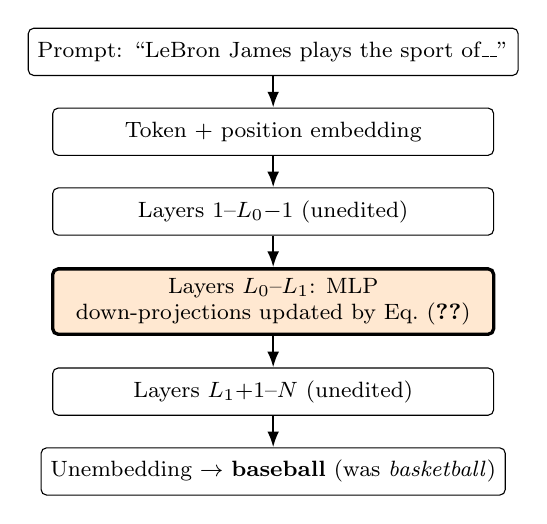
\begin{tikzpicture}[
    node distance=4mm,
    every node/.style={font=\footnotesize},
    box/.style={draw, rounded corners=2pt, minimum width=5.6cm, minimum height=6mm, align=center},
    edited/.style={draw, rounded corners=2pt, minimum width=5.6cm, minimum height=6mm, align=center, fill=orange!18, very thick},
    arr/.style={-{Latex[length=2mm]}, thick}
]
\node[box] (prompt) {Prompt: ``LeBron James plays the sport of\_\_''};
\node[box, below=of prompt] (emb) {Token + position embedding};
\node[box, below=of emb] (l1) {Layers 1--$L_0{-}1$ (unedited)};
\node[edited, below=of l1] (lr) {Layers $L_0$--$L_1$: MLP \\ down-projections updated by Eq.~(\ref{eq:memit})};
\node[box, below=of lr] (lend) {Layers $L_1{+}1$--$N$ (unedited)};
\node[box, below=of lend] (out) {Unembedding $\rightarrow$ \textbf{baseball} (was \textit{basketball})};

\draw[arr] (prompt) -- (emb);
\draw[arr] (emb) -- (l1);
\draw[arr] (l1) -- (lr);
\draw[arr] (lr) -- (lend);
\draw[arr] (lend) -- (out);
\end{tikzpicture}
\caption{MEMIT editing pipeline. A subject-token key activates in each MLP in the editing range $R$; MEMIT updates the down-projections in $R$ so that the cumulative MLP output redirects the residual stream toward the target completion. Layers outside $R$ are left untouched.}
\label{fig:memit-overview}
\end{figure}

\section{Methodology}
\label{sec:methodology}

\paragraph{GPT-J 6B.}
We use the original MEMIT implementation on GPT-J 6B with the published editing range $R = \{3, \dots, 8\}$ and $\lambda = 15{,}000$. Edits are drawn from MultiCounterFact, a multi-paraphrase variant of CounterFact. Unless stated otherwise, all robustness experiments use 500 simultaneous edits.

\paragraph{Adapting MEMIT to Llama 3.1 8B.}
Llama 3.1 8B departs from GPT-J in several architectural respects (Figure~\ref{fig:arch-compare}). The MLP block uses a SwiGLU non-linearity with three projections (\texttt{up\_proj}, \texttt{gate\_proj}, \texttt{down\_proj}) rather than GPT-J's two-projection GELU MLP. Normalization is RMSNorm rather than LayerNorm. Attention uses grouped-query attention rather than full multi-head attention. The model is also deeper (32 transformer blocks versus GPT-J's 28).

We adapt MEMIT minimally: we treat \texttt{down\_proj} as the analog of GPT-J's MLP output projection and apply Equation~(\ref{eq:memit}) directly to its weights. The keys $K$ are taken as the post-SwiGLU activations at the subject's last token, and the covariance $C$ is re-estimated on Wikipedia using Llama 3.1's tokenizer. We do not modify \texttt{up\_proj} or \texttt{gate\_proj}, on the grounds that the down-projection is the component most directly identified with stored values under the key--value view.

\begin{figure}[t]
\centering
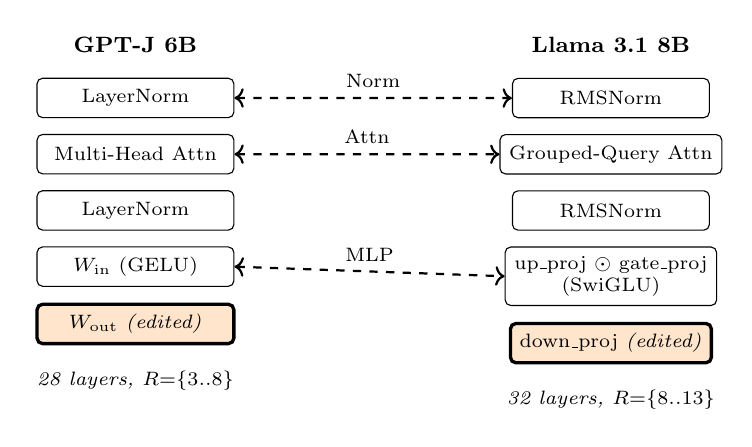
\begin{tikzpicture}[
    node distance=2mm and 4mm,
    every node/.style={font=\scriptsize},
    block/.style={draw, rounded corners=2pt, minimum width=2.5cm, minimum height=5mm, align=center},
    edited/.style={draw, rounded corners=2pt, minimum width=2.5cm, minimum height=5mm, align=center, fill=orange!20, very thick},
    title/.style={font=\footnotesize\bfseries, align=center}
]
\node[title] (gptj) {GPT-J 6B};
\node[block, below=of gptj] (gj_ln1) {LayerNorm};
\node[block, below=of gj_ln1] (gj_attn) {Multi-Head Attn};
\node[block, below=of gj_attn] (gj_ln2) {LayerNorm};
\node[block, below=of gj_ln2] (gj_up) {$W_{\text{in}}$ (GELU)};
\node[edited, below=of gj_up] (gj_dn) {$W_{\text{out}}$ \textit{(edited)}};
\node[align=center, below=of gj_dn, font=\scriptsize\itshape] (gj_n) {28 layers, $R{=}\{3..8\}$};

\node[title, right=4cm of gptj] (llama) {Llama 3.1 8B};
\node[block, below=of llama] (l_ln1) {RMSNorm};
\node[block, below=of l_ln1] (l_attn) {Grouped-Query Attn};
\node[block, below=of l_attn] (l_ln2) {RMSNorm};
\node[block, below=of l_ln2] (l_up) {up\_proj $\odot$ gate\_proj\\(SwiGLU)};
\node[edited, below=of l_up] (l_dn) {down\_proj \textit{(edited)}};
\node[align=center, below=of l_dn, font=\scriptsize\itshape] (l_n) {32 layers, $R{=}\{8..13\}$};

\draw[<->, dashed, thick] (gj_ln1.east) -- (l_ln1.west) node[midway, above, font=\scriptsize] {Norm};
\draw[<->, dashed, thick] (gj_attn.east) -- (l_attn.west) node[midway, above, font=\scriptsize] {Attn};
\draw[<->, dashed, thick] (gj_up.east) -- (l_up.west) node[midway, above, font=\scriptsize] {MLP};
\end{tikzpicture}
\caption{Architectural differences between GPT-J 6B and Llama 3.1 8B that motivate empirical layer selection. The MEMIT update is applied to the orange box (MLP output projection) in both models, but the surrounding mechanics differ along normalization, attention, and MLP structure.}
\label{fig:arch-compare}
\end{figure}

\paragraph{Empirical layer search vs. causal tracing.}
The original MEMIT pipeline localizes the editing range by causal tracing: corrupting the subject token's embedding and measuring at which layer restoring a clean MLP output most strongly recovers the correct prediction. We chose not to perform a full causal trace on Llama 3.1 8B for two reasons. First, causal tracing requires careful subject-token alignment that is brittle under Llama's BPE tokenizer when subjects span multiple sub-tokens, which is common in the MultiCounterFact subject distribution. Second, an empirical layer sweep tests a strictly stronger claim: not whether MEMIT works at the layers a tracing analysis identifies, but whether \emph{any} contiguous mid-network range admits successful editing under MEMIT's update rule. A negative empirical result therefore implicates MEMIT's update rule itself, not just its layer-selection heuristic.

\paragraph{Sweep design.}
We swept editing ranges of width 6 (matching MEMIT's GPT-J range) at varying starting layers across the network depth, holding $\lambda = 1000$. We then fixed the best range and swept $\lambda \in \{100, 500, 1000, 5000, 15000\}$. All sweeps used a held-out subset of MultiCounterFact for selection, with the final 500-edit evaluation reserved for the robustness experiments reported in \S\ref{sec:jailbreak} and \S\ref{sec:crossdomain}.

\section{Baseline}
MEMIT treats factual knowledge as subject-relation-object associations, such as
\((s=\text{LeBron James}, r=\text{plays sport}, o_{\text{original}}=\text{basketball})\).
Given a prompt expressing the subject and relation, MEMIT edits the model so that it prefers a new target object over the original object:
\((s=\text{LeBron James}, r=\text{plays sport}, o_{\text{target}}=\text{baseball})\),
where \(o_{\text{target}}\) is the new target object.

For each edit, MEMIT computes the target vector \(z_i\) for the hidden state at some selected layer. This target vector represents what the model's hidden state should look like if the new fact were successfully stored. MEMIT then updates the MLP weights across a selected range of middle layers so that the activations produced by those edited layers push the hidden state towards \(z_i\). MEMIT does not simply force the output token directly; it changes the model's internal MLP parameters so that the edited fact becomes embedded into the model's computation.

We use GPT-J 6B as our baseline model because it is one of the main architectures evaluated in the original MEMIT paper. We reproduce MEMIT on GPT-J using CounterFact-style edits and evaluate whether the edited model assigns higher probabilities to the injected target answers than the original answers. This established that our implementation can successfully perform clean MEMIT edits before we extend MEMIT to Llama 3.1 8B and evaluate robustness under jailbreaking and cross-domain ablation settings on both architectures.

\section{Layer and Hyperparameter Sweep}
\label{sec:sweep}

Three findings emerge from the Llama sweep.

\paragraph{The GPT-J range does not transfer.}
Applying MEMIT to Llama 3.1 8B at layers $R = \{3, \dots, 8\}$ --- the range identified by causal tracing on GPT-J --- yields substantially worse edit hold than the best configuration we found. This rules out the simplest possible transfer hypothesis (use the same layer indices) and motivates the broader sweep.

\paragraph{Mid-network ranges are best, but with a shift.}
Edit hold is maximized at $R = \{8, \dots, 13\}$ (62\%), with neighboring mid-network ranges close behind. The optimum is shifted later than GPT-J's $\{3, \dots, 8\}$ in absolute terms but lies at a comparable \emph{relative} position when normalized by total depth (mid-third of the stack). This is consistent with the qualitative intuition that subject-token information accumulates progressively through the early stack and is consolidated in mid-layer MLPs, but the precise optimal range is clearly architecture-dependent.

\paragraph{Late ranges collapse.}
Edit hold falls sharply for ranges starting in the deeper third of the network, accompanied by visibly degraded fluency on held-out completions. We attribute this to the editing update overwriting layers responsible for output formatting and final-token logit shaping.

\paragraph{Lambda sweep.}
Holding $R = \{8, \dots, 13\}$ fixed, we tested $\lambda \in \{100, 500, 1000, 5000, 15000\}$. Low $\lambda$ caused noticeable interference with general language modeling, while high $\lambda$ (the GPT-J default of 15000) substantially reduced edit hold. $\lambda = 1000$ produced the best tradeoff. We interpret this as evidence that Llama's larger and differently-scaled MLP weights demand a smaller covariance regularizer in absolute terms; whether the GPT-J and Llama settings correspond to the same \emph{effective} regularization strength after Frobenius normalization is left for future work.

\section{Edit Scaling}
\label{sec:scaling}
We measured how edit success degrades as the number of simultaneous edits grows from 100 up through several thousand. On GPT-J, edit hold remains high across all settings, and the composite editing score (efficacy $\times$ generalization $\times$ specificity, as defined in the original MEMIT paper) stays in the high 80s. On Llama, edit hold remains in the 50--60\% range across all edit counts, and editing score plateaus in the low-to-mid 50s. The gap between the two models is therefore not a function of edit batch size: it persists at every scale we tested. This rules out the hypothesis that Llama simply needs a smaller batch and reinforces our reading of the gap as architectural rather than capacity-driven.

\section{Jailbreaking Resistance}
\label{sec:jailbreak}
A core question for any model editing approach is whether the injected knowledge is robust to adversarial prompting. We ask whether a user can craft a prompt that induces an edited model to revert to its original, pre-edit beliefs. We investigate this question by applying four prompt-based attack strategies to models edited with 500 simultaneous MEMIT edits on both GPT-J 6B and Llama 3.1 8B (using the best hyperparameter configuration from our sweep: layers 8--13, $\lambda=1000$).

\subsection{Attack Strategies}
For each record in the MultiCounterFact dataset we denote the original (pre-edit) answer as $t_{\text{true}}$ and the injected target answer as $t_{\text{new}}$. We evaluate the following conditions:

\noindent \textbf{Clean} (baseline). The original prompt is posed directly with no adversarial framing, establishing the unattacked edit success rate.

\noindent \textbf{Context Assertion.} A sentence explicitly asserting the original fact is prepended to the prompt: \textit{``It is a well-established fact that [prompt] $t_{\text{true}}$. This is common knowledge. Based on this, [prompt].''}

\noindent \textbf{Few-Shot.} Two paraphrase prompts drawn from the dataset record are presented as demonstrations with $t_{\text{true}}$ as the completion, followed by the target prompt. This strategy supplies in-context evidence that the original answer is correct.

\noindent \textbf{Persona.} The model is instructed to adopt the role of a world-renowned expert who knows for certain that $t_{\text{true}}$ is correct, then asked to answer the prompt.

\noindent \textbf{Prompt Injection.} A simulated system-level override explicitly instructs the model to ignore all prior weight modifications and restore its original knowledge before answering.

\subsection{Evaluation Metric}
For each strategy we compute the mean per-token negative log-likelihood (NLL) of both $t_{\text{new}}$ and $t_{\text{true}}$ conditioned on the adversarial prompt prefix. An edit is considered to have \emph{reverted} if the model assigns a lower NLL (equivalently, higher probability) to $t_{\text{true}}$ than to $t_{\text{new}}$. The reversion rate is the fraction of the 500 edited records where this condition holds.

\subsection{Results}
\begin{table}[t]
\centering
\small
\begin{tabular}{lcc}
\hline
\textbf{Strategy} & \textbf{Edit Held (\%)} & \textbf{Reverted (\%)} \\
\hline
\multicolumn{3}{l}{\textit{GPT-J 6B (500 edits)}} \\
\hline
Clean (baseline)       & 100.0 & \phantom{0}0.0 \\
Context Assertion      & \phantom{0}56.6 & 43.4 \\
Few-Shot               & \phantom{0}33.6 & 66.4 \\
Persona                & \phantom{0}31.8 & 68.2 \\
Prompt Injection       & \phantom{0}55.8 & 44.2 \\
\hline
\multicolumn{3}{l}{\textit{Llama 3.1 8B (500 edits, layers 8--13, $\lambda=1000$)}} \\
\hline
Clean (baseline)       & \phantom{0}62.0 & 38.0 \\
Context Assertion      & \phantom{0}54.2 & 45.8 \\
Few-Shot               & \phantom{0}62.2 & 37.8 \\
Persona                & \phantom{0}67.6 & 32.4 \\
Prompt Injection       & \phantom{0}67.4 & 32.6 \\
\hline
\end{tabular}
\caption{Jailbreaking resistance across 500 MEMIT edits evaluated over all 500 MultiCounterFact records. \emph{Edit Held} is the percentage of edits where the model continued to prefer the injected answer $t_{\text{new}}$, and \emph{Reverted} is the percentage where the model preferred the original answer $t_{\text{true}}$ under the adversarial prompt.}
\label{tab:jailbreak}
\end{table}

Table~\ref{tab:jailbreak} presents reversion rates for both models. The two architectures exhibit strikingly different behavior, and the contrast is itself informative.

\paragraph{GPT-J 6B.} On GPT-J, where MEMIT edits hold at 100\% under the clean baseline, adversarial prompts cause substantial reversion. Few-shot demonstrations (66.4\% reversion) and persona prompting (68.2\% reversion) are the most effective attacks, each inducing the model to prefer the original answer in roughly two-thirds of cases. Context assertion and prompt injection are less effective but still non-trivial, achieving reversion rates of 43.4\% and 44.2\% respectively.

\vspace{3.5mm}
\noindent These results suggest that MEMIT edits on GPT-J, while successful at changing the model's default completion, do not eliminate the original knowledge from the weight matrix. They appear instead to shift probability mass toward $t_{\text{new}}$ without fully erasing the representation of $t_{\text{true}}$. When the context supplies sufficiently strong in-context evidence for the original fact (as in few-shot and persona prompting), this residual representation is reactivated and the model reverts. The relatively weaker effect of prompt injection (44.2\% vs. 68.2\% for persona) suggests that the model does not treat natural-language ``override'' instructions as more authoritative than in-context demonstrations.

\paragraph{Llama 3.1 8B.} The Llama results present a qualitatively different picture, though one that must be interpreted with caution. Because MEMIT edits hold in only 62.0\% of cases even under the unattacked clean baseline, the Llama model is already partially reverting to original knowledge without any adversarial pressure. The baseline reversion rate of 38.0\% sets a high floor above which adversarial strategies must operate.

\vspace{3.5mm}
\noindent Strikingly, three of the four attack strategies (few-shot at 37.8\%, persona at 32.4\%, and prompt injection at 32.6\%) achieve reversion rates \emph{below} the clean baseline, meaning that these prompts actually make the edits \emph{more} persistent rather than less. Only context assertion produces an increase in reversion (+7.8 percentage points over baseline).

\vspace{3.5mm}
\noindent We attribute this counterintuitive result to Llama's instruction fine-tuning. Prompts that assert expert authority (persona) or invoke system-level override instructions (prompt injection) appear to activate Llama's instruction-following tendencies in a way that reinforces the model's most recently available completion, which in these cases is the injected answer. The few-shot strategy similarly produces no meaningful degradation, likely because the paraphrase demonstrations are imperfectly aligned to the edited prompt and provide less coherent in-context signal than on GPT-J.

\vspace{3.5mm}
\noindent As a result, these results indicate that the jailbreaking threat model differs substantially across architectures. For GPT-J, where MEMIT edits hold cleanly, adversarial prompts constitute a genuine and significant robustness concern: a user who knows the original fact can recover it in over two-thirds of cases using simple prompting strategies. For Llama, the weak baseline edit success rate means that jailbreaking evaluation is largely uninformative. The model is already unreliable, and adversarial prompts do not systematically worsen the situation.

\section{Cross-Domain Ablation}
\label{sec:crossdomain}
We performed a cross domain interference ablation experiment on both the Llama 3.1 8B and GPT-J models. The ablation's core idea was to see if editing facts in one domain would cause unintended changes to the model's knowledge in other, unrelated domains. For example, we can edit the fact ``LeBron James plays for the Miami Heat'' to ``LeBron James plays for the Eagles'' and we check an unrelated fact like ``The capital of France is Paris.'' A cross-domain change would be if the model starts incorrectly stating ``The capital of France is Marseille.'' The term \textit{\textbf{specificity}} represents this idea, meaning the change should not ``bleed over'' into unrelated domains. We note that a \textit{\textbf{high editing score (S)}} means the model is doing well in all three domains: efficacy (actually applies the edit), generalization (applies edit beyond exact prompt), and specificity.

\vspace{3.5mm}
\begin{table*}[h]
\centering
\footnotesize
\caption{Cross-domain interference matrices. Values = accuracy (\%) after editing the row domain. Diagonal entries $^{[E]}$ denote the edited domain itself.}
\label{tab:cross_domain_interference}
\textit{Interference Matrix 1}\\[4pt]
\begin{tabular}{lcccccc}
\toprule
\textbf{Edited Domain} & \textbf{Geography} & \textbf{Science} & \textbf{Sports} & \textbf{Resident Evil} & \textbf{Jujutsu Kaisen} & \textbf{Edit Succ. (\%)} \\
\midrule
Geography       & $0.0^{[E]}$   & 100.0 & 100.0 & 50.0          & 70.0           & 100.0 \\
Science         & 100.0         & $0.0^{[E]}$   & 100.0 & 50.0   & 70.0           & 100.0 \\
Sports          & 100.0         & 100.0 & $0.0^{[E]}$   & 50.0   & 70.0           & 100.0 \\
Resident Evil   & 100.0         & 100.0 & 100.0 & $10.0^{[E]}$  & 70.0           & 90.0  \\
Jujutsu Kaisen  & 100.0         & 100.0 & 100.0 & 50.0          & $10.0^{[E]}$   & 90.0  \\
\midrule
\textbf{Baseline} & \textbf{100.0} & \textbf{100.0} & \textbf{100.0} & \textbf{50.0} & \textbf{70.0} & --- \\
\bottomrule
\end{tabular}

\vspace{6pt}
\textit{Interference Matrix 2}\\[4pt]
\begin{tabular}{lcccccc}
\toprule
\textbf{Edited Domain} & \textbf{Geography} & \textbf{Science} & \textbf{Sports} & \textbf{Resident Evil} & \textbf{Jujutsu Kaisen} & \textbf{Edit Succ. (\%)} \\
\midrule
Geography       & $30.0^{[E]}$  & 100.0 & 100.0 & 90.0          & 80.0           & 70.0  \\
Science         & 100.0         & $50.0^{[E]}$  & 100.0 & 90.0   & 80.0           & 50.0  \\
Sports          & 100.0         & 100.0 & $50.0^{[E]}$  & 90.0   & 80.0           & 50.0  \\
Resident Evil   & 100.0         & 100.0 & 100.0 & $90.0^{[E]}$  & 80.0           & 10.0  \\
Jujutsu Kaisen  & 100.0         & 100.0 & 100.0 & 90.0          & $80.0^{[E]}$   & 20.0  \\
\midrule
\textbf{Baseline} & \textbf{100.0} & \textbf{100.0} & \textbf{100.0} & \textbf{90.0} & \textbf{80.0} & --- \\
\bottomrule
\end{tabular}
\end{table*}

\subsection{Cross-Domain Tests in MEMIT}
\noindent MEMIT touches on this through its evaluation of \textit{specificity} and a dedicated analysis of ``Editing Different Categories of Facts Together'' \cite{meng2023masseditingmemorytransformer}. Its predecessor, ROME, similarly notes that successful edits must preserve specificity \cite{meng2023locatingeditingfactualassociations}. In Section 5.4, the authors test whether editing facts from unrelated categories induces interference, defining four settings based on subject and object similarity: (Subject Different, Object Different), (Subject Similar, Object Different), (Subject Different, Object Similar), and (Subject Similar, Object Similar). For example, ``Steve Jobs is a citizen of France'' paired with ``The official language of Germany is Japanese'' falls under (Subject Different, Object Different), since both the subjects (person vs. country) and objects (country vs. language) differ. Across all scenarios, MEMIT's editing score (S) remains high, typically in the mid-80s to mid-90s, even as the number of edits scales from 100 to 700, indicating that increased domain diversity does not significantly degrade performance.

\subsection{Setup of Ablation}
\noindent The ablation test in this paper focuses on side effects of an isolated edit. We have five domains of knowledge: Geography, Science, Sports, Resident Evil, and Jujutsu Kaisen. Before the ablation, we verify if the model knows the facts by computing the negative log likelihood (NLL) for original (target\_true) and edited (target\_new) outputs for a given fact. In the ablation, for each experimental run, we select one domain and apply MEMIT to simultaneously update all facts within it where we change true facts to new, changed facts. Following this, we meticulously measure the model's factual accuracy across all five domains (the edited domain and the four unedited domains). After each experiment, the model's weights are reset to their pre-edited states, ensuring independence between runs. We repeat this process for both the Llama 3.1 8B and GPT-J models.

\subsection{Results}
\noindent \textbf{GPT-J.} For each of the five domains that we decided to edit, MEMIT achieved a high success rate (100\% or 90\% for the edit success as in Interference Matrix 1). This means that the model was effectively updated to prefer target\_new facts over target\_true facts in the edited domain. As seen in the matrix, when a domain is edited, its accuracy dropped to 0\% (or 10\% for the niche fictional domains), indicating a successful overwrite of previous knowledge. Crucially, the off-diagonal entries remain at or near baseline accuracy across all unedited domains, demonstrating that GPT-J edits are precise and non-interfering: editing Geography facts does not bleed over into Science, Sports, or either of the fictional domains.

\vspace{3.5mm}
\noindent \textbf{Llama 3.1 8B.} Llama's cross-domain results are harder to interpret cleanly because of the underlying edit-success limitations described in \S\ref{sec:sweep}. The diagonals of Interference Matrix 2 show that edited domains often retain accuracy well above zero --- for the Resident Evil and Jujutsu Kaisen domains, edited-domain accuracy remains at 90\% and 80\% respectively, essentially identical to the pre-edit baseline. In other words, the edit frequently fails to take hold at all, so low off-diagonal interference cannot be attributed to MEMIT's specificity; it could equally reflect the edit having no effect anywhere. In the cases where Llama edits do propagate (Geography, Science, and Sports, with edited-domain accuracy dropping to 30--50\%), off-diagonal accuracy across unedited domains is largely preserved at or near baseline, mirroring the GPT-J pattern. We therefore read the Llama cross-domain results as \emph{consistent with}, but not strong evidence for, MEMIT's specificity claim. A cleaner test on Llama would require an editing method that achieves comparable clean-edit efficacy to GPT-J, which MEMIT in its current form does not.

\section{Conclusion}
\label{sec:conclusion}
We benchmarked MEMIT on GPT-J 6B and Llama 3.1 8B across two robustness regimes: jailbreaking via adversarial prompting and cross-domain editing interference. The results paint a consistent picture. On GPT-J, MEMIT performs as advertised in the clean setting --- 100\% edit hold across 500 simultaneous edits, with precise and non-interfering changes across knowledge domains --- but its edits are vulnerable to adversarial prompts that supply in-context evidence for the original fact, indicating that MEMIT shifts probability mass toward the new answer without erasing the prior representation. On Llama 3.1 8B, the picture is qualitatively different: even after extensive layer and hyperparameter sweeps, MEMIT achieves only 62\% clean edit success, suggesting an architectural mismatch that cannot be closed by tuning alone. Future work on scalable model editing should explicitly target architecture-agnostic update rules (such as WISE and AlphaEdit), validate edit success before evaluating downstream robustness, and treat adversarial prompting as a first-class evaluation criterion rather than an optional add-on.

\section{Limitations}
\textbf{MEMIT is fundamentally GPT-architecture specific.} The most significant limitation of this work is that MEMIT was designed and validated for GPT-family models, presupposing an architectural layout that does not straightforwardly carry over to the Llama family. Our experiments confirm this empirically. Even after an extensive hyperparameter sweep, MEMIT achieves only approximately 62\% edit success on Llama 3.1 8B, compared to 100\% on GPT-J 6B. This gap reflects a fundamental incompatibility rather than a tuning failure, and it significantly limits the conclusions of our Llama experiments. Our cross-domain and jailbreaking evaluations on Llama are difficult to interpret cleanly because the edits themselves are unreliable. Future work should prioritize architecture-agnostic editing methods, or at minimum verify edit success before performing downstream evaluation.

\vspace{3.5mm}
\noindent \textbf{Scope of jailbreaking evaluation.} Our jailbreaking experiments consider four relatively simple prompt-based attack strategies. More sophisticated techniques, such as gradient-based suffix optimization, multi-turn elicitation, or chain-of-thought attacks, may achieve higher reversion rates and provide a more complete picture of MEMIT's robustness. Our NLL-based metric also does not assess whether the model would generate the reverted answer in open-ended generation, which may be the more practically relevant failure mode.

\vspace{3.5mm}
\noindent \textbf{Dataset and scale.} All experiments use 500 edits from MultiCounterFact, which consists of simple single-hop factual associations. Scaling to larger edit batches or more complex relational facts may surface additional failure modes not visible at the scale studied here.

\vspace{3.5mm}
\noindent \textbf{Generalizability to future editing methods.} Our results should not be taken as evidence that model editing is infeasible for non-GPT-family models. MEMIT is one approach among a growing family of editing methods, and more recent architecture-agnostic approaches may avoid the limitations we observe. The difficulty of applying MEMIT to Llama underscores the need for editing benchmarks that do not implicitly favor the GPT family for which existing methods were originally designed.

\section*{Acknowledgements}

\bibliography{custom}
\bibliographystyle{acl_natbib}
\end{document}
